% compile with pdflatex -shell-escape file.tex
\documentclass[convert={density=300,outext=.png}]{standalone}
\usepackage{tikz}
\usetikzlibrary{calc,fit,positioning}
\usetikzlibrary{decorations.markings}
\usetikzlibrary{backgrounds}
\usetikzlibrary{shapes}

% Fibre node style
\makeatletter
\tikzset{
  fibre node/.style={
    draw, ellipse, align=center
  },
  reset transform/.code={\pgftransformreset}
}
\makeatother

\begin{document}
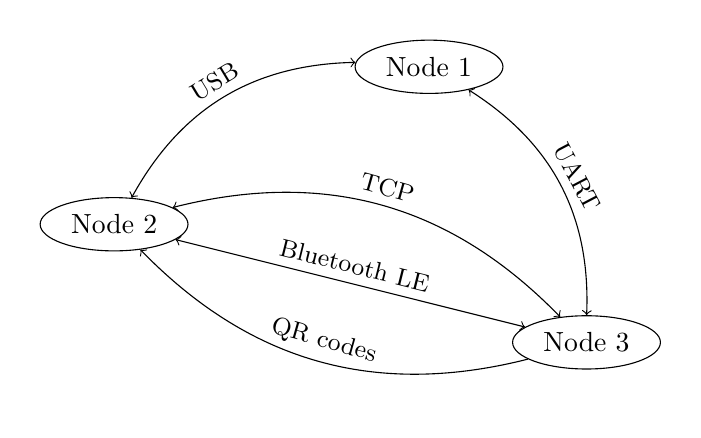
\begin{tikzpicture}[background rectangle/.style={fill=white!45}, show background rectangle]
    \draw (4,2) node[fibre node] (node1) {Node 1};
    \draw (0,0) node[fibre node] (node2) {Node 2};
    \draw (6,-1.5) node[fibre node] (node3) {Node 3};
    \draw (node1) edge[<->, bend right] node[sloped,midway,above] {\small USB} (node2);
    \draw (node2) edge[<->, bend left] node[sloped,midway,above] {\small TCP} (node3);
    \draw (node2) edge[<->] node[sloped,midway,above] {\small Bluetooth LE} (node3);
    \draw (node2) edge[<-, bend right] node[sloped,midway,above] {\small QR codes} (node3);
    \draw (node1) edge[<->, bend left] node[sloped,midway,above] {\small UART} (node3);
\end{tikzpicture}
\end{document}